\documentclass[nolineno]{ieeeaccess}
\usepackage[T1]{fontenc}
\usepackage{amsmath,amssymb,amsthm,booktabs,array,graphicx}
\usepackage{cite,xurl,etoolbox,float,enumitem,needspace}
\usepackage[hidelinks]{hyperref}
\graphicspath{{../../research/r7c/figures/}}
% Research-draft metadata only; retain the class's typography and page geometry (as in R6).
\makeatletter
\patchcmd{\@maketitle}{Digital Object Identifier\space\@doi}{}{}{\PackageError{inarcp}{Cannot suppress unassigned DOI}{Check the IEEE Access class version.}}
\patchcmd{\thebibliography}{\addcontentsline{toc}{section}{\refname}}{\phantomsection\addcontentsline{toc}{section}{\refname}}{}{\PackageError{inarcp}{Cannot anchor bibliography}{Check the IEEE Access class version.}}
\def\ps@inarcpdraft{\def\@oddhead{}\def\@evenhead{}%
  \def\@oddfoot{\hfil\footerpagefont\thepage\hfil}%
  \let\@evenfoot\@oddfoot}
\let\ps@firstpage\ps@inarcpdraft
\let\ps@titlepage\ps@inarcpdraft
\let\ps@headings\ps@inarcpdraft
\makeatother
\pagestyle{inarcpdraft}
\raggedbottom
\newlength{\inarcpabstractwidth}
\setlength{\inarcpabstractwidth}{\dimexpr\titlewidth-10pt\relax}
\let\abstractwidth\inarcpabstractwidth
\makeatletter\input{t1pcr.fd}\makeatother
\DeclareFontShape{T1}{pcr}{n}{n}{<->ssub*pcr/m/n}{}
\newtheorem{proposition}{Proposition}
\newtheorem{corollary}{Corollary}
\newcommand{\PP}{\mathbb{P}}
\newcommand{\BelowGOnemEightA}{5}
\newcommand{\BelowGOnemEightB}{0}
\newcommand{\BelowGOnemSixteenA}{4}
\newcommand{\BelowGOnemSixteenB}{0}
\newcommand{\BelowINFourmEightA}{5}
\newcommand{\BelowINFourmEightB}{0}
\newcommand{\BelowINFourmSixteenA}{9}
\newcommand{\BelowINFourmSixteenB}{0}
\newcommand{\BelowINOnemEightA}{0}
\newcommand{\BelowINOnemEightB}{0}
\newcommand{\BelowINOnemSixteenA}{7}
\newcommand{\BelowINOnemSixteenB}{0}
\newcommand{\BelowINTwomEightA}{7}
\newcommand{\BelowINTwomEightB}{0}
\newcommand{\BelowINTwomSixteenA}{4}
\newcommand{\BelowINTwomSixteenB}{0}
\newcommand{\BelowLSmEightA}{2}
\newcommand{\BelowLSmEightB}{0}
\newcommand{\BelowLSmSixteenA}{4}
\newcommand{\BelowLSmSixteenB}{0}
\newcommand{\BelowMLPmEightA}{21}
\newcommand{\BelowMLPmEightB}{0}
\newcommand{\BelowMLPmSixteenA}{21}
\newcommand{\BelowMLPmSixteenB}{0}
\newcommand{\BelowMONmEightA}{4}
\newcommand{\BelowMONmEightB}{0}
\newcommand{\BelowMONmSixteenA}{7}
\newcommand{\BelowMONmSixteenB}{0}
\newcommand{\BelowNAFourGmEightA}{66}
\newcommand{\BelowNAFourGmEightB}{2}
\newcommand{\BelowNAFourGmSixteenA}{29}
\newcommand{\BelowNAFourGmSixteenB}{2}
\newcommand{\BelowNAFourmEightA}{5}
\newcommand{\BelowNAFourmEightB}{0}
\newcommand{\BelowNAFourmSixteenA}{11}
\newcommand{\BelowNAFourmSixteenB}{0}
\newcommand{\BelowNAOneGmEightA}{62}
\newcommand{\BelowNAOneGmEightB}{0}
\newcommand{\BelowNAOneGmSixteenA}{45}
\newcommand{\BelowNAOneGmSixteenB}{2}
\newcommand{\BelowNAOnemEightA}{2}
\newcommand{\BelowNAOnemEightB}{0}
\newcommand{\BelowNAOnemSixteenA}{9}
\newcommand{\BelowNAOnemSixteenB}{0}
\newcommand{\BelowNATwomEightA}{5}
\newcommand{\BelowNATwomEightB}{0}
\newcommand{\BelowNATwomSixteenA}{9}
\newcommand{\BelowNATwomSixteenB}{0}
\newcommand{\BelowRMSmEightA}{29}
\newcommand{\BelowRMSmEightB}{0}
\newcommand{\BelowRMSmSixteenA}{20}
\newcommand{\BelowRMSmSixteenB}{4}
\newcommand{\BelowUmEightA}{25}
\newcommand{\BelowUmEightB}{5}
\newcommand{\BelowUmSixteenA}{21}
\newcommand{\BelowUmSixteenB}{5}
\newcommand{\CFiveCorrA}{0.86}
\newcommand{\CFiveCorrB}{0.96}
\newcommand{\CFiveMaeA}{0.0090}
\newcommand{\CFiveMaeB}{0.0012}
\newcommand{\CFiveNaiveA}{0.0156}
\newcommand{\CFiveNaiveB}{0.0042}
\newcommand{\CleanGOnemEightA}{1.012}
\newcommand{\CleanGOnemEightB}{1.028}
\newcommand{\CleanGOnemSixteenA}{0.997}
\newcommand{\CleanGOnemSixteenB}{0.992}
\newcommand{\CleanINFourmEightA}{0.848}
\newcommand{\CleanINFourmEightB}{0.933}
\newcommand{\CleanINFourmSixteenA}{0.802}
\newcommand{\CleanINFourmSixteenB}{0.820}
\newcommand{\CleanINOnemEightA}{1.000}
\newcommand{\CleanINOnemEightB}{1.000}
\newcommand{\CleanINOnemSixteenA}{1.000}
\newcommand{\CleanINOnemSixteenB}{1.000}
\newcommand{\CleanINTwomEightA}{0.878}
\newcommand{\CleanINTwomEightB}{0.932}
\newcommand{\CleanINTwomSixteenA}{0.865}
\newcommand{\CleanINTwomSixteenB}{0.873}
\newcommand{\CleanLSmEightA}{0.859}
\newcommand{\CleanLSmEightB}{0.967}
\newcommand{\CleanLSmSixteenA}{0.871}
\newcommand{\CleanLSmSixteenB}{1.018}
\newcommand{\CleanMLPmEightA}{1.378}
\newcommand{\CleanMLPmEightB}{1.862}
\newcommand{\CleanMLPmSixteenA}{1.390}
\newcommand{\CleanMLPmSixteenB}{1.740}
\newcommand{\CleanMONmEightA}{0.953}
\newcommand{\CleanMONmEightB}{0.952}
\newcommand{\CleanMONmSixteenA}{0.980}
\newcommand{\CleanMONmSixteenB}{1.002}
\newcommand{\CleanNAFourGmEightA}{0.666}
\newcommand{\CleanNAFourGmEightB}{0.626}
\newcommand{\CleanNAFourGmSixteenA}{0.682}
\newcommand{\CleanNAFourGmSixteenB}{0.654}
\newcommand{\CleanNAFourmEightA}{0.706}
\newcommand{\CleanNAFourmEightB}{0.695}
\newcommand{\CleanNAFourmSixteenA}{0.709}
\newcommand{\CleanNAFourmSixteenB}{0.704}
\newcommand{\CleanNAOneGmEightA}{0.927}
\newcommand{\CleanNAOneGmEightB}{0.873}
\newcommand{\CleanNAOneGmSixteenA}{0.952}
\newcommand{\CleanNAOneGmSixteenB}{0.913}
\newcommand{\CleanNAOnemEightA}{0.985}
\newcommand{\CleanNAOnemEightB}{0.982}
\newcommand{\CleanNAOnemSixteenA}{0.989}
\newcommand{\CleanNAOnemSixteenB}{0.984}
\newcommand{\CleanNATwomEightA}{0.738}
\newcommand{\CleanNATwomEightB}{0.731}
\newcommand{\CleanNATwomSixteenA}{0.739}
\newcommand{\CleanNATwomSixteenB}{0.738}
\newcommand{\CleanRMSmEightA}{1.480}
\newcommand{\CleanRMSmEightB}{1.930}
\newcommand{\CleanRMSmSixteenA}{1.404}
\newcommand{\CleanRMSmSixteenB}{1.729}
\newcommand{\CleanUmEightA}{1.065}
\newcommand{\CleanUmEightB}{1.660}
\newcommand{\CleanUmSixteenA}{1.073}
\newcommand{\CleanUmSixteenB}{1.700}
\newcommand{\CovGOnemEightA}{0.903}
\newcommand{\CovGOnemEightB}{0.991}
\newcommand{\CovGOnemSixteenA}{0.900}
\newcommand{\CovGOnemSixteenB}{0.990}
\newcommand{\CovINFourmEightA}{0.901}
\newcommand{\CovINFourmEightB}{0.991}
\newcommand{\CovINFourmSixteenA}{0.901}
\newcommand{\CovINFourmSixteenB}{0.990}
\newcommand{\CovINOnemEightA}{0.902}
\newcommand{\CovINOnemEightB}{0.991}
\newcommand{\CovINOnemSixteenA}{0.901}
\newcommand{\CovINOnemSixteenB}{0.990}
\newcommand{\CovINTwomEightA}{0.901}
\newcommand{\CovINTwomEightB}{0.991}
\newcommand{\CovINTwomSixteenA}{0.901}
\newcommand{\CovINTwomSixteenB}{0.990}
\newcommand{\CovLSmEightA}{0.899}
\newcommand{\CovLSmEightB}{0.990}
\newcommand{\CovLSmSixteenA}{0.900}
\newcommand{\CovLSmSixteenB}{0.991}
\newcommand{\CovMLPmEightA}{0.898}
\newcommand{\CovMLPmEightB}{0.990}
\newcommand{\CovMLPmSixteenA}{0.901}
\newcommand{\CovMLPmSixteenB}{0.990}
\newcommand{\CovMONmEightA}{0.903}
\newcommand{\CovMONmEightB}{0.993}
\newcommand{\CovMONmSixteenA}{0.904}
\newcommand{\CovMONmSixteenB}{0.992}
\newcommand{\CovMinGOnemEightA}{0.860}
\newcommand{\CovMinGOnemEightB}{0.978}
\newcommand{\CovMinGOnemSixteenA}{0.845}
\newcommand{\CovMinGOnemSixteenB}{0.979}
\newcommand{\CovMinINFourmEightA}{0.873}
\newcommand{\CovMinINFourmEightB}{0.982}
\newcommand{\CovMinINFourmSixteenA}{0.869}
\newcommand{\CovMinINFourmSixteenB}{0.978}
\newcommand{\CovMinINOnemEightA}{0.880}
\newcommand{\CovMinINOnemEightB}{0.980}
\newcommand{\CovMinINOnemSixteenA}{0.864}
\newcommand{\CovMinINOnemSixteenB}{0.973}
\newcommand{\CovMinINTwomEightA}{0.862}
\newcommand{\CovMinINTwomEightB}{0.983}
\newcommand{\CovMinINTwomSixteenA}{0.871}
\newcommand{\CovMinINTwomSixteenB}{0.982}
\newcommand{\CovMinLSmEightA}{0.878}
\newcommand{\CovMinLSmEightB}{0.982}
\newcommand{\CovMinLSmSixteenA}{0.866}
\newcommand{\CovMinLSmSixteenB}{0.981}
\newcommand{\CovMinMLPmEightA}{0.854}
\newcommand{\CovMinMLPmEightB}{0.979}
\newcommand{\CovMinMLPmSixteenA}{0.850}
\newcommand{\CovMinMLPmSixteenB}{0.977}
\newcommand{\CovMinMONmEightA}{0.873}
\newcommand{\CovMinMONmEightB}{0.982}
\newcommand{\CovMinMONmSixteenA}{0.862}
\newcommand{\CovMinMONmSixteenB}{0.984}
\newcommand{\CovMinNAFourGmEightA}{0.806}
\newcommand{\CovMinNAFourGmEightB}{0.968}
\newcommand{\CovMinNAFourGmSixteenA}{0.811}
\newcommand{\CovMinNAFourGmSixteenB}{0.964}
\newcommand{\CovMinNAFourmEightA}{0.873}
\newcommand{\CovMinNAFourmEightB}{0.983}
\newcommand{\CovMinNAFourmSixteenA}{0.853}
\newcommand{\CovMinNAFourmSixteenB}{0.980}
\newcommand{\CovMinNAOneGmEightA}{0.805}
\newcommand{\CovMinNAOneGmEightB}{0.972}
\newcommand{\CovMinNAOneGmSixteenA}{0.812}
\newcommand{\CovMinNAOneGmSixteenB}{0.968}
\newcommand{\CovMinNAOnemEightA}{0.877}
\newcommand{\CovMinNAOnemEightB}{0.980}
\newcommand{\CovMinNAOnemSixteenA}{0.855}
\newcommand{\CovMinNAOnemSixteenB}{0.975}
\newcommand{\CovMinNATwomEightA}{0.866}
\newcommand{\CovMinNATwomEightB}{0.980}
\newcommand{\CovMinNATwomSixteenA}{0.861}
\newcommand{\CovMinNATwomSixteenB}{0.978}
\newcommand{\CovMinRMSmEightA}{0.861}
\newcommand{\CovMinRMSmEightB}{0.979}
\newcommand{\CovMinRMSmSixteenA}{0.845}
\newcommand{\CovMinRMSmSixteenB}{0.963}
\newcommand{\CovMinUmEightA}{0.781}
\newcommand{\CovMinUmEightB}{0.949}
\newcommand{\CovMinUmSixteenA}{0.801}
\newcommand{\CovMinUmSixteenB}{0.967}
\newcommand{\CovNAFourGmEightA}{0.873}
\newcommand{\CovNAFourGmEightB}{0.982}
\newcommand{\CovNAFourGmSixteenA}{0.885}
\newcommand{\CovNAFourGmSixteenB}{0.985}
\newcommand{\CovNAFourmEightA}{0.900}
\newcommand{\CovNAFourmEightB}{0.990}
\newcommand{\CovNAFourmSixteenA}{0.902}
\newcommand{\CovNAFourmSixteenB}{0.991}
\newcommand{\CovNAOneGmEightA}{0.874}
\newcommand{\CovNAOneGmEightB}{0.981}
\newcommand{\CovNAOneGmSixteenA}{0.882}
\newcommand{\CovNAOneGmSixteenB}{0.984}
\newcommand{\CovNAOnemEightA}{0.901}
\newcommand{\CovNAOnemEightB}{0.991}
\newcommand{\CovNAOnemSixteenA}{0.901}
\newcommand{\CovNAOnemSixteenB}{0.990}
\newcommand{\CovNATwomEightA}{0.900}
\newcommand{\CovNATwomEightB}{0.991}
\newcommand{\CovNATwomSixteenA}{0.901}
\newcommand{\CovNATwomSixteenB}{0.991}
\newcommand{\CovRMSmEightA}{0.899}
\newcommand{\CovRMSmEightB}{0.991}
\newcommand{\CovRMSmSixteenA}{0.899}
\newcommand{\CovRMSmSixteenB}{0.989}
\newcommand{\CovUmEightA}{0.899}
\newcommand{\CovUmEightB}{0.989}
\newcommand{\CovUmSixteenA}{0.899}
\newcommand{\CovUmSixteenB}{0.989}
\newcommand{\CurveHighGOnemEightA}{0.918}
\newcommand{\CurveHighGOnemEightB}{0.995}
\newcommand{\CurveHighGOnemSixteenA}{0.908}
\newcommand{\CurveHighGOnemSixteenB}{0.993}
\newcommand{\CurveHighINFourmEightA}{0.902}
\newcommand{\CurveHighINFourmEightB}{0.992}
\newcommand{\CurveHighINFourmSixteenA}{0.903}
\newcommand{\CurveHighINFourmSixteenB}{0.991}
\newcommand{\CurveHighINOnemEightA}{0.917}
\newcommand{\CurveHighINOnemEightB}{0.994}
\newcommand{\CurveHighINOnemSixteenA}{0.908}
\newcommand{\CurveHighINOnemSixteenB}{0.993}
\newcommand{\CurveHighINTwomEightA}{0.902}
\newcommand{\CurveHighINTwomEightB}{0.993}
\newcommand{\CurveHighINTwomSixteenA}{0.902}
\newcommand{\CurveHighINTwomSixteenB}{0.990}
\newcommand{\CurveHighLSmEightA}{0.883}
\newcommand{\CurveHighLSmEightB}{0.986}
\newcommand{\CurveHighLSmSixteenA}{0.890}
\newcommand{\CurveHighLSmSixteenB}{0.987}
\newcommand{\CurveHighMLPmEightA}{0.948}
\newcommand{\CurveHighMLPmEightB}{0.997}
\newcommand{\CurveHighMLPmSixteenA}{0.950}
\newcommand{\CurveHighMLPmSixteenB}{0.995}
\newcommand{\CurveHighMONmEightA}{0.878}
\newcommand{\CurveHighMONmEightB}{0.988}
\newcommand{\CurveHighMONmSixteenA}{0.887}
\newcommand{\CurveHighMONmSixteenB}{0.989}
\newcommand{\CurveHighNAFourGmEightA}{0.863}
\newcommand{\CurveHighNAFourGmEightB}{0.978}
\newcommand{\CurveHighNAFourGmSixteenA}{0.880}
\newcommand{\CurveHighNAFourGmSixteenB}{0.981}
\newcommand{\CurveHighNAFourmEightA}{0.890}
\newcommand{\CurveHighNAFourmEightB}{0.988}
\newcommand{\CurveHighNAFourmSixteenA}{0.898}
\newcommand{\CurveHighNAFourmSixteenB}{0.988}
\newcommand{\CurveHighNAOneGmEightA}{0.887}
\newcommand{\CurveHighNAOneGmEightB}{0.986}
\newcommand{\CurveHighNAOneGmSixteenA}{0.894}
\newcommand{\CurveHighNAOneGmSixteenB}{0.987}
\newcommand{\CurveHighNAOnemEightA}{0.915}
\newcommand{\CurveHighNAOnemEightB}{0.993}
\newcommand{\CurveHighNAOnemSixteenA}{0.911}
\newcommand{\CurveHighNAOnemSixteenB}{0.992}
\newcommand{\CurveHighNATwomEightA}{0.898}
\newcommand{\CurveHighNATwomEightB}{0.991}
\newcommand{\CurveHighNATwomSixteenA}{0.905}
\newcommand{\CurveHighNATwomSixteenB}{0.989}
\newcommand{\CurveHighRMSmEightA}{0.951}
\newcommand{\CurveHighRMSmEightB}{0.997}
\newcommand{\CurveHighRMSmSixteenA}{0.957}
\newcommand{\CurveHighRMSmSixteenB}{0.997}
\newcommand{\CurveHighUmEightA}{0.741}
\newcommand{\CurveHighUmEightB}{0.954}
\newcommand{\CurveHighUmSixteenA}{0.744}
\newcommand{\CurveHighUmSixteenB}{0.953}
\newcommand{\CurveLowGOnemEightA}{0.889}
\newcommand{\CurveLowGOnemEightB}{0.989}
\newcommand{\CurveLowGOnemSixteenA}{0.894}
\newcommand{\CurveLowGOnemSixteenB}{0.988}
\newcommand{\CurveLowINFourmEightA}{0.900}
\newcommand{\CurveLowINFourmEightB}{0.990}
\newcommand{\CurveLowINFourmSixteenA}{0.900}
\newcommand{\CurveLowINFourmSixteenB}{0.989}
\newcommand{\CurveLowINOnemEightA}{0.889}
\newcommand{\CurveLowINOnemEightB}{0.988}
\newcommand{\CurveLowINOnemSixteenA}{0.896}
\newcommand{\CurveLowINOnemSixteenB}{0.988}
\newcommand{\CurveLowINTwomEightA}{0.902}
\newcommand{\CurveLowINTwomEightB}{0.991}
\newcommand{\CurveLowINTwomSixteenA}{0.899}
\newcommand{\CurveLowINTwomSixteenB}{0.989}
\newcommand{\CurveLowLSmEightA}{0.909}
\newcommand{\CurveLowLSmEightB}{0.992}
\newcommand{\CurveLowLSmSixteenA}{0.908}
\newcommand{\CurveLowLSmSixteenB}{0.992}
\newcommand{\CurveLowMLPmEightA}{0.824}
\newcommand{\CurveLowMLPmEightB}{0.980}
\newcommand{\CurveLowMLPmSixteenA}{0.818}
\newcommand{\CurveLowMLPmSixteenB}{0.977}
\newcommand{\CurveLowMONmEightA}{0.927}
\newcommand{\CurveLowMONmEightB}{0.996}
\newcommand{\CurveLowMONmSixteenA}{0.921}
\newcommand{\CurveLowMONmSixteenB}{0.995}
\newcommand{\CurveLowNAFourGmEightA}{0.893}
\newcommand{\CurveLowNAFourGmEightB}{0.986}
\newcommand{\CurveLowNAFourGmSixteenA}{0.899}
\newcommand{\CurveLowNAFourGmSixteenB}{0.987}
\newcommand{\CurveLowNAFourmEightA}{0.918}
\newcommand{\CurveLowNAFourmEightB}{0.993}
\newcommand{\CurveLowNAFourmSixteenA}{0.916}
\newcommand{\CurveLowNAFourmSixteenB}{0.993}
\newcommand{\CurveLowNAOneGmEightA}{0.865}
\newcommand{\CurveLowNAOneGmEightB}{0.978}
\newcommand{\CurveLowNAOneGmSixteenA}{0.877}
\newcommand{\CurveLowNAOneGmSixteenB}{0.981}
\newcommand{\CurveLowNAOnemEightA}{0.895}
\newcommand{\CurveLowNAOnemEightB}{0.989}
\newcommand{\CurveLowNAOnemSixteenA}{0.898}
\newcommand{\CurveLowNAOnemSixteenB}{0.988}
\newcommand{\CurveLowNATwomEightA}{0.910}
\newcommand{\CurveLowNATwomEightB}{0.991}
\newcommand{\CurveLowNATwomSixteenA}{0.907}
\newcommand{\CurveLowNATwomSixteenB}{0.991}
\newcommand{\CurveLowRMSmEightA}{0.820}
\newcommand{\CurveLowRMSmEightB}{0.981}
\newcommand{\CurveLowRMSmSixteenA}{0.812}
\newcommand{\CurveLowRMSmSixteenB}{0.974}
\newcommand{\CurveLowUmEightA}{0.982}
\newcommand{\CurveLowUmEightB}{0.999}
\newcommand{\CurveLowUmSixteenA}{0.978}
\newcommand{\CurveLowUmSixteenB}{0.999}
\newcommand{\HoCovGOne}{0.945}
\newcommand{\HoCovINFour}{0.906}
\newcommand{\HoCovINOne}{0.910}
\newcommand{\HoCovINTwo}{0.906}
\newcommand{\HoCovLS}{0.919}
\newcommand{\HoCovMLP}{0.903}
\newcommand{\HoCovMON}{0.896}
\newcommand{\HoCovNAFour}{0.893}
\newcommand{\HoCovNAFourG}{0.856}
\newcommand{\HoCovNAOne}{0.903}
\newcommand{\HoCovNATwo}{0.895}
\newcommand{\HoCovRMS}{0.887}
\newcommand{\HoCovU}{0.859}
\newcommand{\HoMonInf}{infinite}
\newcommand{\HoRatioGOne}{1.104}
\newcommand{\HoRatioINFour}{0.515}
\newcommand{\HoRatioINOne}{1.000}
\newcommand{\HoRatioINTwo}{0.572}
\newcommand{\HoRatioLS}{0.662}
\newcommand{\HoRatioMLP}{2.158}
\newcommand{\HoRatioMON}{0.981}
\newcommand{\HoRatioNAFour}{0.498}
\newcommand{\HoRatioNAFourG}{0.472}
\newcommand{\HoRatioNAOne}{0.921}
\newcommand{\HoRatioNATwo}{0.533}
\newcommand{\HoRatioRMS}{1.243}
\newcommand{\HoRatioU}{1.161}
\newcommand{\MaxdevGOnemEightA}{0.038}
\newcommand{\MaxdevGOnemEightB}{0.011}
\newcommand{\MaxdevGOnemSixteenA}{0.034}
\newcommand{\MaxdevGOnemSixteenB}{0.011}
\newcommand{\MaxdevINFourmEightA}{0.031}
\newcommand{\MaxdevINFourmEightB}{0.010}
\newcommand{\MaxdevINFourmSixteenA}{0.032}
\newcommand{\MaxdevINFourmSixteenB}{0.011}
\newcommand{\MaxdevINOneWFiveTwelve}{0.035}
\newcommand{\MaxdevINOneWTwentyFortyEight}{0.033}
\newcommand{\MaxdevINOnemEightA}{0.037}
\newcommand{\MaxdevINOnemEightB}{0.011}
\newcommand{\MaxdevINOnemSixteenA}{0.036}
\newcommand{\MaxdevINOnemSixteenB}{0.011}
\newcommand{\MaxdevINTwomEightA}{0.035}
\newcommand{\MaxdevINTwomEightB}{0.010}
\newcommand{\MaxdevINTwomSixteenA}{0.034}
\newcommand{\MaxdevINTwomSixteenB}{0.010}
\newcommand{\MaxdevLSmEightA}{0.039}
\newcommand{\MaxdevLSmEightB}{0.012}
\newcommand{\MaxdevLSmSixteenA}{0.039}
\newcommand{\MaxdevLSmSixteenB}{0.012}
\newcommand{\MaxdevMLPWFiveTwelve}{0.103}
\newcommand{\MaxdevMLPWTwentyFortyEight}{0.080}
\newcommand{\MaxdevMLPmEightA}{0.092}
\newcommand{\MaxdevMLPmEightB}{0.015}
\newcommand{\MaxdevMLPmSixteenA}{0.096}
\newcommand{\MaxdevMLPmSixteenB}{0.019}
\newcommand{\MaxdevMONWFiveTwelve}{0.042}
\newcommand{\MaxdevMONWTwentyFortyEight}{0.039}
\newcommand{\MaxdevMONmEightA}{0.043}
\newcommand{\MaxdevMONmEightB}{0.010}
\newcommand{\MaxdevMONmSixteenA}{0.043}
\newcommand{\MaxdevMONmSixteenB}{0.011}
\newcommand{\MaxdevNAFourGmEightA}{0.063}
\newcommand{\MaxdevNAFourGmEightB}{0.020}
\newcommand{\MaxdevNAFourGmSixteenA}{0.049}
\newcommand{\MaxdevNAFourGmSixteenB}{0.016}
\newcommand{\MaxdevNAFourWFiveTwelve}{0.043}
\newcommand{\MaxdevNAFourWTwentyFortyEight}{0.043}
\newcommand{\MaxdevNAFourmEightA}{0.043}
\newcommand{\MaxdevNAFourmEightB}{0.010}
\newcommand{\MaxdevNAFourmSixteenA}{0.043}
\newcommand{\MaxdevNAFourmSixteenB}{0.011}
\newcommand{\MaxdevNAOneGmEightA}{0.062}
\newcommand{\MaxdevNAOneGmEightB}{0.021}
\newcommand{\MaxdevNAOneGmSixteenA}{0.051}
\newcommand{\MaxdevNAOneGmSixteenB}{0.017}
\newcommand{\MaxdevNAOnemEightA}{0.043}
\newcommand{\MaxdevNAOnemEightB}{0.012}
\newcommand{\MaxdevNAOnemSixteenA}{0.042}
\newcommand{\MaxdevNAOnemSixteenB}{0.011}
\newcommand{\MaxdevNATwomEightA}{0.042}
\newcommand{\MaxdevNATwomEightB}{0.011}
\newcommand{\MaxdevNATwomSixteenA}{0.044}
\newcommand{\MaxdevNATwomSixteenB}{0.011}
\newcommand{\MaxdevRMSWFiveTwelve}{0.110}
\newcommand{\MaxdevRMSWTwentyFortyEight}{0.086}
\newcommand{\MaxdevRMSmEightA}{0.096}
\newcommand{\MaxdevRMSmEightB}{0.015}
\newcommand{\MaxdevRMSmSixteenA}{0.103}
\newcommand{\MaxdevRMSmSixteenB}{0.021}
\newcommand{\MaxdevUWFiveTwelve}{0.181}
\newcommand{\MaxdevUWTwentyFortyEight}{0.141}
\newcommand{\MaxdevUmEightA}{0.170}
\newcommand{\MaxdevUmEightB}{0.038}
\newcommand{\MaxdevUmSixteenA}{0.165}
\newcommand{\MaxdevUmSixteenB}{0.039}
\newcommand{\NUnitsConf}{56}
\newcommand{\NoisyGOnemEightA}{0.979}
\newcommand{\NoisyGOnemEightB}{0.949}
\newcommand{\NoisyGOnemSixteenA}{0.990}
\newcommand{\NoisyGOnemSixteenB}{0.993}
\newcommand{\NoisyINFourmEightA}{0.986}
\newcommand{\NoisyINFourmEightB}{1.228}
\newcommand{\NoisyINFourmSixteenA}{0.953}
\newcommand{\NoisyINFourmSixteenB}{0.964}
\newcommand{\NoisyINOnemEightA}{1.000}
\newcommand{\NoisyINOnemEightB}{1.000}
\newcommand{\NoisyINOnemSixteenA}{1.000}
\newcommand{\NoisyINOnemSixteenB}{1.000}
\newcommand{\NoisyINTwomEightA}{0.977}
\newcommand{\NoisyINTwomEightB}{1.008}
\newcommand{\NoisyINTwomSixteenA}{0.968}
\newcommand{\NoisyINTwomSixteenB}{0.957}
\newcommand{\NoisyLSmEightA}{0.997}
\newcommand{\NoisyLSmEightB}{1.093}
\newcommand{\NoisyLSmSixteenA}{1.046}
\newcommand{\NoisyLSmSixteenB}{1.207}
\newcommand{\NoisyMLPmEightA}{1.178}
\newcommand{\NoisyMLPmEightB}{1.227}
\newcommand{\NoisyMLPmSixteenA}{1.224}
\newcommand{\NoisyMLPmSixteenB}{1.278}
\newcommand{\NoisyMONmEightA}{0.953}
\newcommand{\NoisyMONmEightB}{0.905}
\newcommand{\NoisyMONmSixteenA}{0.980}
\newcommand{\NoisyMONmSixteenB}{0.987}
\newcommand{\NoisyNAFourGmEightA}{0.804}
\newcommand{\NoisyNAFourGmEightB}{0.722}
\newcommand{\NoisyNAFourGmSixteenA}{0.839}
\newcommand{\NoisyNAFourGmSixteenB}{0.811}
\newcommand{\NoisyNAFourmEightA}{0.839}
\newcommand{\NoisyNAFourmEightB}{0.758}
\newcommand{\NoisyNAFourmSixteenA}{0.866}
\newcommand{\NoisyNAFourmSixteenB}{0.840}
\newcommand{\NoisyNAOneGmEightA}{0.851}
\newcommand{\NoisyNAOneGmEightB}{0.764}
\newcommand{\NoisyNAOneGmSixteenA}{0.882}
\newcommand{\NoisyNAOneGmSixteenB}{0.853}
\newcommand{\NoisyNAOnemEightA}{0.897}
\newcommand{\NoisyNAOnemEightB}{0.823}
\newcommand{\NoisyNAOnemSixteenA}{0.915}
\newcommand{\NoisyNAOnemSixteenB}{0.884}
\newcommand{\NoisyNATwomEightA}{0.845}
\newcommand{\NoisyNATwomEightB}{0.763}
\newcommand{\NoisyNATwomSixteenA}{0.871}
\newcommand{\NoisyNATwomSixteenB}{0.843}
\newcommand{\NoisyRMSmEightA}{1.274}
\newcommand{\NoisyRMSmEightB}{1.302}
\newcommand{\NoisyRMSmSixteenA}{1.288}
\newcommand{\NoisyRMSmSixteenB}{1.363}
\newcommand{\NoisyUmEightA}{0.962}
\newcommand{\NoisyUmEightB}{0.951}
\newcommand{\NoisyUmSixteenA}{0.994}
\newcommand{\NoisyUmSixteenB}{1.066}
\newcommand{\RatioGOnemEightA}{1.001}
\newcommand{\RatioGOnemEightB}{1.002}
\newcommand{\RatioGOnemSixteenA}{0.995}
\newcommand{\RatioGOnemSixteenB}{0.993}
\newcommand{\RatioHiGOnemEightA}{1.013}
\newcommand{\RatioHiGOnemEightB}{1.031}
\newcommand{\RatioHiGOnemSixteenA}{1.002}
\newcommand{\RatioHiGOnemSixteenB}{1.005}
\newcommand{\RatioHiINFourmEightA}{0.957}
\newcommand{\RatioHiINFourmEightB}{1.142}
\newcommand{\RatioHiINFourmSixteenA}{0.905}
\newcommand{\RatioHiINFourmSixteenB}{0.918}
\newcommand{\RatioHiINOnemEightA}{1.000}
\newcommand{\RatioHiINOnemEightB}{1.000}
\newcommand{\RatioHiINOnemSixteenA}{1.000}
\newcommand{\RatioHiINOnemSixteenB}{1.000}
\newcommand{\RatioHiINTwomEightA}{0.965}
\newcommand{\RatioHiINTwomEightB}{1.007}
\newcommand{\RatioHiINTwomSixteenA}{0.953}
\newcommand{\RatioHiINTwomSixteenB}{0.953}
\newcommand{\RatioHiLSmEightA}{0.958}
\newcommand{\RatioHiLSmEightB}{1.064}
\newcommand{\RatioHiLSmSixteenA}{0.990}
\newcommand{\RatioHiLSmSixteenB}{1.147}
\newcommand{\RatioHiMLPmEightA}{1.416}
\newcommand{\RatioHiMLPmEightB}{1.839}
\newcommand{\RatioHiMLPmSixteenA}{1.439}
\newcommand{\RatioHiMLPmSixteenB}{1.780}
\newcommand{\RatioHiMONmEightA}{0.963}
\newcommand{\RatioHiMONmEightB}{0.958}
\newcommand{\RatioHiMONmSixteenA}{0.984}
\newcommand{\RatioHiMONmSixteenB}{1.006}
\newcommand{\RatioHiNAFourGmEightA}{0.764}
\newcommand{\RatioHiNAFourGmEightB}{0.697}
\newcommand{\RatioHiNAFourGmSixteenA}{0.787}
\newcommand{\RatioHiNAFourGmSixteenB}{0.758}
\newcommand{\RatioHiNAFourmEightA}{0.800}
\newcommand{\RatioHiNAFourmEightB}{0.738}
\newcommand{\RatioHiNAFourmSixteenA}{0.815}
\newcommand{\RatioHiNAFourmSixteenB}{0.798}
\newcommand{\RatioHiNAOneGmEightA}{0.931}
\newcommand{\RatioHiNAOneGmEightB}{0.876}
\newcommand{\RatioHiNAOneGmSixteenA}{0.958}
\newcommand{\RatioHiNAOneGmSixteenB}{0.920}
\newcommand{\RatioHiNAOnemEightA}{0.988}
\newcommand{\RatioHiNAOnemEightB}{0.989}
\newcommand{\RatioHiNAOnemSixteenA}{0.994}
\newcommand{\RatioHiNAOnemSixteenB}{0.989}
\newcommand{\RatioHiNATwomEightA}{0.808}
\newcommand{\RatioHiNATwomEightB}{0.752}
\newcommand{\RatioHiNATwomSixteenA}{0.824}
\newcommand{\RatioHiNATwomSixteenB}{0.806}
\newcommand{\RatioHiRMSmEightA}{1.507}
\newcommand{\RatioHiRMSmEightB}{1.871}
\newcommand{\RatioHiRMSmSixteenA}{1.449}
\newcommand{\RatioHiRMSmSixteenB}{1.782}
\newcommand{\RatioHiUmEightA}{1.071}
\newcommand{\RatioHiUmEightB}{1.627}
\newcommand{\RatioHiUmSixteenA}{1.085}
\newcommand{\RatioHiUmSixteenB}{1.720}
\newcommand{\RatioINFourmEightA}{0.890}
\newcommand{\RatioINFourmEightB}{1.019}
\newcommand{\RatioINFourmSixteenA}{0.845}
\newcommand{\RatioINFourmSixteenB}{0.861}
\newcommand{\RatioINOnemEightA}{1.000}
\newcommand{\RatioINOnemEightB}{1.000}
\newcommand{\RatioINOnemSixteenA}{1.000}
\newcommand{\RatioINOnemSixteenB}{1.000}
\newcommand{\RatioINTwomEightA}{0.909}
\newcommand{\RatioINTwomEightB}{0.956}
\newcommand{\RatioINTwomSixteenA}{0.895}
\newcommand{\RatioINTwomSixteenB}{0.898}
\newcommand{\RatioLSmEightA}{0.901}
\newcommand{\RatioLSmEightB}{1.005}
\newcommand{\RatioLSmSixteenA}{0.921}
\newcommand{\RatioLSmSixteenB}{1.072}
\newcommand{\RatioLoGOnemEightA}{0.987}
\newcommand{\RatioLoGOnemEightB}{0.968}
\newcommand{\RatioLoGOnemSixteenA}{0.988}
\newcommand{\RatioLoGOnemSixteenB}{0.979}
\newcommand{\RatioLoINFourmEightA}{0.844}
\newcommand{\RatioLoINFourmEightB}{0.935}
\newcommand{\RatioLoINFourmSixteenA}{0.805}
\newcommand{\RatioLoINFourmSixteenB}{0.822}
\newcommand{\RatioLoINOnemEightA}{1.000}
\newcommand{\RatioLoINOnemEightB}{1.000}
\newcommand{\RatioLoINOnemSixteenA}{1.000}
\newcommand{\RatioLoINOnemSixteenB}{1.000}
\newcommand{\RatioLoINTwomEightA}{0.867}
\newcommand{\RatioLoINTwomEightB}{0.918}
\newcommand{\RatioLoINTwomSixteenA}{0.855}
\newcommand{\RatioLoINTwomSixteenB}{0.857}
\newcommand{\RatioLoLSmEightA}{0.863}
\newcommand{\RatioLoLSmEightB}{0.968}
\newcommand{\RatioLoLSmSixteenA}{0.875}
\newcommand{\RatioLoLSmSixteenB}{1.019}
\newcommand{\RatioLoMLPmEightA}{1.257}
\newcommand{\RatioLoMLPmEightB}{1.475}
\newcommand{\RatioLoMLPmSixteenA}{1.288}
\newcommand{\RatioLoMLPmSixteenB}{1.489}
\newcommand{\RatioLoMONmEightA}{0.941}
\newcommand{\RatioLoMONmEightB}{0.909}
\newcommand{\RatioLoMONmSixteenA}{0.975}
\newcommand{\RatioLoMONmSixteenB}{0.988}
\newcommand{\RatioLoNAFourGmEightA}{0.672}
\newcommand{\RatioLoNAFourGmEightB}{0.629}
\newcommand{\RatioLoNAFourGmSixteenA}{0.687}
\newcommand{\RatioLoNAFourGmSixteenB}{0.659}
\newcommand{\RatioLoNAFourmEightA}{0.713}
\newcommand{\RatioLoNAFourmEightB}{0.701}
\newcommand{\RatioLoNAFourmSixteenA}{0.714}
\newcommand{\RatioLoNAFourmSixteenB}{0.706}
\newcommand{\RatioLoNAOneGmEightA}{0.866}
\newcommand{\RatioLoNAOneGmEightB}{0.787}
\newcommand{\RatioLoNAOneGmSixteenA}{0.895}
\newcommand{\RatioLoNAOneGmSixteenB}{0.860}
\newcommand{\RatioLoNAOnemEightA}{0.913}
\newcommand{\RatioLoNAOnemEightB}{0.853}
\newcommand{\RatioLoNAOnemSixteenA}{0.930}
\newcommand{\RatioLoNAOnemSixteenB}{0.907}
\newcommand{\RatioLoNATwomEightA}{0.747}
\newcommand{\RatioLoNATwomEightB}{0.724}
\newcommand{\RatioLoNATwomSixteenA}{0.748}
\newcommand{\RatioLoNATwomSixteenB}{0.745}
\newcommand{\RatioLoRMSmEightA}{1.364}
\newcommand{\RatioLoRMSmEightB}{1.565}
\newcommand{\RatioLoRMSmSixteenA}{1.320}
\newcommand{\RatioLoRMSmSixteenB}{1.533}
\newcommand{\RatioLoUmEightA}{0.985}
\newcommand{\RatioLoUmEightB}{1.140}
\newcommand{\RatioLoUmSixteenA}{1.010}
\newcommand{\RatioLoUmSixteenB}{1.261}
\newcommand{\RatioMLPmEightA}{1.310}
\newcommand{\RatioMLPmEightB}{1.628}
\newcommand{\RatioMLPmSixteenA}{1.337}
\newcommand{\RatioMLPmSixteenB}{1.585}
\newcommand{\RatioMONmEightA}{0.953}
\newcommand{\RatioMONmEightB}{0.936}
\newcommand{\RatioMONmSixteenA}{0.980}
\newcommand{\RatioMONmSixteenB}{0.998}
\newcommand{\RatioNAFourGmEightA}{0.707}
\newcommand{\RatioNAFourGmEightB}{0.656}
\newcommand{\RatioNAFourGmSixteenA}{0.726}
\newcommand{\RatioNAFourGmSixteenB}{0.698}
\newcommand{\RatioNAFourmEightA}{0.746}
\newcommand{\RatioNAFourmEightB}{0.715}
\newcommand{\RatioNAFourmSixteenA}{0.753}
\newcommand{\RatioNAFourmSixteenB}{0.743}
\newcommand{\RatioNAOneGmEightA}{0.902}
\newcommand{\RatioNAOneGmEightB}{0.836}
\newcommand{\RatioNAOneGmSixteenA}{0.930}
\newcommand{\RatioNAOneGmSixteenB}{0.894}
\newcommand{\RatioNAOnemEightA}{0.955}
\newcommand{\RatioNAOnemEightB}{0.928}
\newcommand{\RatioNAOnemSixteenA}{0.966}
\newcommand{\RatioNAOnemSixteenB}{0.952}
\newcommand{\RatioNATwomEightA}{0.771}
\newcommand{\RatioNATwomEightB}{0.741}
\newcommand{\RatioNATwomSixteenA}{0.777}
\newcommand{\RatioNATwomSixteenB}{0.769}
\newcommand{\RatioRMSmEightA}{1.410}
\newcommand{\RatioRMSmEightB}{1.701}
\newcommand{\RatioRMSmSixteenA}{1.368}
\newcommand{\RatioRMSmSixteenB}{1.609}
\newcommand{\RatioUmEightA}{1.031}
\newcommand{\RatioUmEightB}{1.388}
\newcommand{\RatioUmSixteenA}{1.048}
\newcommand{\RatioUmSixteenB}{1.475}
\newcommand{\RefGOnemEightA}{0.029}
\newcommand{\RefGOnemEightB}{0.009}
\newcommand{\RefGOnemSixteenA}{0.029}
\newcommand{\RefGOnemSixteenB}{0.009}
\newcommand{\RefINFourmEightA}{0.029}
\newcommand{\RefINFourmEightB}{0.009}
\newcommand{\RefINFourmSixteenA}{0.029}
\newcommand{\RefINFourmSixteenB}{0.009}
\newcommand{\RefINOnemEightA}{0.029}
\newcommand{\RefINOnemEightB}{0.009}
\newcommand{\RefINOnemSixteenA}{0.029}
\newcommand{\RefINOnemSixteenB}{0.009}
\newcommand{\RefINTwomEightA}{0.029}
\newcommand{\RefINTwomEightB}{0.009}
\newcommand{\RefINTwomSixteenA}{0.029}
\newcommand{\RefINTwomSixteenB}{0.009}
\newcommand{\RefLSmEightA}{0.029}
\newcommand{\RefLSmEightB}{0.009}
\newcommand{\RefLSmSixteenA}{0.029}
\newcommand{\RefLSmSixteenB}{0.009}
\newcommand{\RefMLPmEightA}{0.029}
\newcommand{\RefMLPmEightB}{0.009}
\newcommand{\RefMLPmSixteenA}{0.029}
\newcommand{\RefMLPmSixteenB}{0.009}
\newcommand{\RefMONmEightA}{0.029}
\newcommand{\RefMONmEightB}{0.009}
\newcommand{\RefMONmSixteenA}{0.029}
\newcommand{\RefMONmSixteenB}{0.009}
\newcommand{\RefNAFourGmEightA}{0.029}
\newcommand{\RefNAFourGmEightB}{0.009}
\newcommand{\RefNAFourGmSixteenA}{0.029}
\newcommand{\RefNAFourGmSixteenB}{0.009}
\newcommand{\RefNAFourmEightA}{0.029}
\newcommand{\RefNAFourmEightB}{0.009}
\newcommand{\RefNAFourmSixteenA}{0.029}
\newcommand{\RefNAFourmSixteenB}{0.009}
\newcommand{\RefNAOneGmEightA}{0.029}
\newcommand{\RefNAOneGmEightB}{0.009}
\newcommand{\RefNAOneGmSixteenA}{0.029}
\newcommand{\RefNAOneGmSixteenB}{0.009}
\newcommand{\RefNAOnemEightA}{0.029}
\newcommand{\RefNAOnemEightB}{0.009}
\newcommand{\RefNAOnemSixteenA}{0.029}
\newcommand{\RefNAOnemSixteenB}{0.009}
\newcommand{\RefNATwomEightA}{0.029}
\newcommand{\RefNATwomEightB}{0.009}
\newcommand{\RefNATwomSixteenA}{0.029}
\newcommand{\RefNATwomSixteenB}{0.009}
\newcommand{\RefRMSmEightA}{0.029}
\newcommand{\RefRMSmEightB}{0.009}
\newcommand{\RefRMSmSixteenA}{0.029}
\newcommand{\RefRMSmSixteenB}{0.009}
\newcommand{\RefUmEightA}{0.029}
\newcommand{\RefUmEightB}{0.009}
\newcommand{\RefUmSixteenA}{0.029}
\newcommand{\RefUmSixteenB}{0.009}
\newcommand{\SynNaGCov}{0.884}
\newcommand{\SynNaHigh}{0.899}
\newcommand{\SynNaLow}{0.904}
\newcommand{\SynNaRatio}{0.949}
\newcommand{\SynNoiseInHigh}{0.909}
\newcommand{\SynNoiseInLow}{0.890}
\newcommand{\SynNoiseMaxT}{1.72}
\newcommand{\SynNoiseMonHigh}{0.882}
\newcommand{\SynNoiseMonLow}{0.926}
\newcommand{\SynNuHat}{1.000}
\newcommand{\SynReps}{200}
\newcommand{\SynRhoHat}{0.930}
\newcommand{\SynSirvInHigh}{0.901}
\newcommand{\SynSirvInLow}{0.900}
\newcommand{\SynSirvMaxT}{1.39}
\newcommand{\SynSirvMonHigh}{0.885}
\newcommand{\SynSirvMonLow}{0.912}
\newcommand{\TrRatioINFour}{0.993}
\newcommand{\TrRatioINOne}{1.000}
\newcommand{\TrRatioLS}{0.967}
\newcommand{\TrRatioMLP}{1.200}
\newcommand{\TrRatioNAFour}{0.936}
\newcommand{\TrRatioNAFourG}{0.893}
\newcommand{\TrRatioRMS}{1.466}
\newcommand{\TrRatioU}{1.470}
\newcommand{\TrWorstINFour}{0.894}
\newcommand{\TrWorstINOne}{0.882}
\newcommand{\TrWorstLS}{0.774}
\newcommand{\TrWorstMLP}{0.622}
\newcommand{\TrWorstNAFour}{0.863}
\newcommand{\TrWorstNAFourG}{0.842}
\newcommand{\TrWorstRMS}{0.681}
\newcommand{\TrWorstU}{0.716}

\begin{document}
\history{}
\doi{}
% WORKING TITLE -- final title is the authors' decision.
\title{Texture-Invariant Conformal Prediction for Compound-Gaussian Autoregressive Clutter: Exact Coverage Laws, Thermal Noise and Sea-Clutter Evaluation}
\author{\uppercase{Muhammad Umair Raza}\authorrefmark{1},
\uppercase{Sohail Ahmed}\authorrefmark{2}, and
\uppercase{Ammad Ahmed}\authorrefmark{3}}
\address[1]{Department of Avionics Engineering, College of Aeronautical Engineering, National University of Sciences and Technology, Risalpur, Pakistan}
\address[2]{MathWorks, United States}
\address[3]{NDMA, Pakistan}
\corresp{Corresponding author: Muhammad Umair Raza (e-mail: uraza@cae.nust.edu.pk).}
\begin{abstract}
Radar clutter episodes share short-term speckle dynamics but differ strongly in amplitude (texture). A calibrated one-step prediction region for such episodes should therefore hold its coverage conditionally on the texture, which is the CFAR-type requirement, and not only on average. We study split-conformal prediction discs for complex compound-Gaussian autoregressive episodes with additive thermal noise.

For any fitted autoregressive predictor, the coverage of an innovation-normalized score has an elementary exact law obtained from complex quadratic forms. Under pure compound-Gaussian clutter this law is texture-free; under thermal noise it gives the exact coverage as a function of the clutter-to-noise ratio. We also show that calibrating within bins of a history-estimated scale (Mondrian calibration) tilts coverage conditional on the latent texture, with explicit signed limits. We propose a noise-aware normalization: a clutter-plus-noise model is fitted with a nonparametric texture distribution, each episode's clutter-to-noise ratio is estimated from its history, and the Gaussian predictive score is calibrated conformally. It reduces to the innovation-normalized score when the noise vanishes.

On 14 IPIX sea-clutter sessions, analysed under a pre-registered protocol with confirmatory rotations and two held-out sessions, the noise-aware AR(4) disc has \RatioNAFourmSixteenA{} times the radius of the innovation-normalized AR(1) baseline (95\% CI \RatioLoNAFourmSixteenA--\RatioHiNAFourmSixteenA), with coverage \CovNAFourmSixteenA{} at nominal 0.90. Its Gaussian plug-in under-covers (\CovNAFourGmSixteenA). Unnormalized, raw-RMS and neural-centre conformal baselines lose texture-conditional coverage. The gains require same-session training data; across days the innovation-normalized construction is the most robust.
\end{abstract}
\begin{keywords}
Conformal prediction, compound-Gaussian clutter, sea clutter, K-distribution, thermal noise, autoregressive models, prediction regions, CFAR.
\end{keywords}
\maketitle

\section{Introduction}
Sea and land clutter observed by a coherent radar is commonly described as compound Gaussian. A slowly varying texture scales locally Gaussian speckle whose correlation reflects the Doppler spectrum, and thermal noise adds a floor \cite{ward2013,conte1995,ollila2012}. Short episodes of the complex returns from one range cell therefore share their standardized dynamics while their amplitudes differ by tens of decibels. A prediction region for the next return that is useful for monitoring, suppression or anomaly screening must be calibrated. It must also be calibrated \emph{for every texture level}; otherwise its false-exceedance rate depends on the clutter power. This is the constant-false-alarm-rate (CFAR) requirement in prediction form.

Recent sea-clutter predictors, including recurrent, encoder--decoder and attention-based networks, report point-prediction error or suppression gain \cite{ma2019,qu2023,li2025taes}. To our knowledge, none provides calibrated prediction regions or reports empirical coverage. Conformal prediction supplies finite-sample marginal coverage for exchangeable data \cite{lei2018}, but its conditional behaviour depends on the score \cite{barber2021limits,gibbs2025,dewolf2025}. In radar it has so far been used for prediction sets in SAR target recognition \cite{spie2025}. Adjacent signal-processing uses include wireless communications \cite{cohen2023}, and conformal $p$-values provide a natural CFAR-type analogue \cite{bates2023}. To our knowledge, it has not been applied to clutter I/Q forecasting.

Our previous analysis of innovation-normalized autoregressive conformal prediction (IN-ARCP) for real-valued AR(1) episodes derived its exact expected length and its fitting and calibration costs. Those efficiency effects are small, and that study was synthetic. Here we turn to the problem the construction is suited to, complex radar clutter, and to real data. The contributions are as follows.
\begin{enumerate}[leftmargin=*,itemsep=2pt]
\item \textbf{Exact coverage laws.} For a complex innovation-normalized score at any fitted predictor, coverage has an elementary exact law (Proposition~\ref{prop:law}), a specialization of classical quadratic-form theory. It shows that the construction is texture-free under compound-Gaussian clutter. It also gives the exact coverage as a function of the clutter-to-noise ratio under thermal noise and, via the known Beta representation, under calibration-to-test shift.
\item \textbf{A latent-versus-observed conditioning result.} Proposition~\ref{prop:mondrian} shows that calibrating within bins of a history-estimated scale tilts coverage conditional on the latent texture, with explicit signed limits, whereas per-episode equivariant normalization is exactly flat.
\item \textbf{Noise-aware normalization.} The proposed score uses a likelihood-fitted clutter-plus-noise model with a nonparametric texture distribution and per-episode clutter-to-noise estimation, and it contains IN-ARCP as its zero-noise limit (Proposition~\ref{prop:reduce}).
\item \textbf{A pre-registered real-data study.} On IPIX sea clutter we report width, marginal coverage, texture-conditional coverage, day transfer, exact coverage prediction and a one-time hold-out. The comparison includes classical Gaussian thresholds and flexible conformal baselines, and unfavourable outcomes are reported.
\end{enumerate}

\section{Related Work}
\subsection{Conformal prediction and conditional validity}
Split conformal prediction gives marginal coverage for exchangeable data and normalized scores adapt interval width \cite{lei2018}. Exact distribution-free conditional coverage is impossible in general \cite{barber2021limits}. Guarantees over finite-dimensional classes of shifts or groups are possible \cite{gibbs2025}, and so is Mondrian calibration within observed categories \cite{vovk2012,bostrom2020}. For location--scale families, a standardized score is pivotal, and normalized conformal prediction is then conditionally valid \cite{dewolf2025}. Dewolf et al.\ also note that taxonomies built on estimated quantities mix the true classes \cite{dewolf2025}; Proposition~\ref{prop:mondrian} makes the resulting latent-conditional tilt explicit for a texture. A post-processing view of conditional validity through pivotal scores is given in \cite{laplante2026}.

Expected conformal set size and the training/calibration trade-off have general treatments \cite{dhillon2024,das2026,yao2026}. Split conformal prediction for a single dependent series is analysed in \cite{barber2026,zhai2026}. The beta representation of calibration-conditional coverage is classical \cite{vovk2012}, and its use under shift appears in \cite{ramos2026}. Under-coverage of plug-in predictive limits with estimated parameters is also classical \cite{barndorff1996,lawless2005,vidoni2009}.

\subsection{Compound-Gaussian clutter and normalized statistics}
Scale invariance of normalized detectors under compound-Gaussian clutter underlies texture-CFAR detection \cite{conte1995,kraut1999,ollila2012}. The parametric and normalized parametric adaptive matched filters whiten with an AR model and normalize by the whitened power \cite{roman2000,michels2000}; our IN-ARCP score applies the same normalization to one-step prediction. Thermal noise alters the clutter statistics and the behaviour of normalized detectors, which is the K+noise regime \cite{watts1987,ward2013}. Structured and robust estimation of the speckle correlation under unknown texture is established \cite{tyler1987,hallin2006}. We use a likelihood fit with a nonparametric texture distribution because the conformal step, not the estimator, carries the validity guarantee.

% R7 manuscript body: model, method, theory, experiments, results, discussion.
% Every numeric result is a macro from generated/r7_macros.tex (make_generated.py).

\section{Model and Prediction Regions}
\subsection{Compound-Gaussian autoregressive episodes with thermal noise}
An episode is $X=(H_1,\dots,H_m,Y)\in\mathbb{C}^{m+1}$: $m$ consecutive complex (I/Q) samples of one range cell and the next sample $Y$ to be predicted. Conditional on a latent texture, the episode is circular complex Gaussian,
\begin{equation}
X\mid c\sim\mathcal{CN}\big(0,\ \nu\,(cR+I)\big),
\label{eq:r7model}
\end{equation}
where $R$ is the unit-diagonal speckle correlation matrix, $\nu\ge0$ is the thermal-noise power and $c>0$ is the clutter-to-noise ratio (CNR) of that episode. With $\nu=0$ and $\nu c\equiv\sigma^2$ fixed, \eqref{eq:r7model} is the compound-Gaussian (spherically invariant) clutter model \cite{conte1995,ollila2012}; the additive term is the thermal noise of the K+noise description of sea clutter \cite{watts1987,ward2013}. The speckle is modelled as a stationary complex AR($p$) process, so that $R$ is determined by $p$ complex reflection coefficients; a nonzero phase represents the mean Doppler shift. Episodes from disjoint times or range cells are the sampling units; the rank argument requires calibration and test episodes to be exchangeable.

\subsection{Normalized prediction discs}
Every procedure in this paper outputs a disc
\begin{equation}
C(h)=\{y\in\mathbb C:\ |y-\mu(h)|\le \widehat q\,s(h)\},
\label{eq:disc}
\end{equation}
with a centre $\mu$ and a positive scale $s$ fitted on training episodes, and $\widehat q$ the $\lceil(n+1)(1-\alpha)\rceil$-th smallest calibration score $|Y_i-\mu(H_i)|/s(H_i)$ over $n$ separate calibration episodes. Split-conformal rank arguments then give marginal coverage at least $1-\alpha$ for exchangeable calibration and test episodes \cite{lei2018}.

\emph{IN-ARCP} (the R6 construction, complexified) uses the pooled least-squares AR(1) coefficient $r$, the centre $rh_m$ and the innovation scale $s_r(h)^2=m^{-1}\{(1-|r|^2)|h_1|^2+\sum_{j\ge2}|h_j-rh_{j-1}|^2\}$. The AR($p$) variant uses the pooled least-squares AR($p$) predictor and the root mean square of the $m-p$ conditional history innovations. Both scales are homogeneous of degree one in the episode, so the score is invariant to the episode amplitude. The construction is analogous to, though not identical with, the AR whitening and whitened-power normalization of the (normalized) parametric adaptive matched filter \cite{roman2000,michels2000}; here it is applied to one-step prediction rather than detection.

\subsection{Noise-aware normalization}
When $\nu>0$ the innovation scale no longer cancels the texture, because the noise floor makes the standardized dynamics depend on $c$. The noise-aware (NA) procedure replaces it by the Gaussian predictive distribution of \eqref{eq:r7model}:
\begin{enumerate}[leftmargin=*,itemsep=2pt]
\item \textbf{Clutter+noise fit.} On training episodes, maximize the marginal likelihood of \eqref{eq:r7model} over the AR($p$) reflection coefficients, $\log\nu$, and a nonparametric texture distribution supported on a fixed CNR grid. The texture weights are profiled by EM (a discrete nonparametric maximum-likelihood estimate); the outer optimization is Nelder--Mead.
\item \textbf{Per-episode CNR.} For each history $h$, $\widehat c(h)$ maximizes the likelihood of $h$ alone under $\mathcal{CN}(0,\widehat\nu(cR_H+I))$.
\item \textbf{Predictive disc.} $\mu(h)$ and $s(h)^2$ are the Gaussian conditional mean and variance of $Y$ given $h$ at $c=\widehat c(h)$; $\widehat q$ is calibrated conformally.
\end{enumerate}
This is a model-based instance of normalized conformal prediction \cite{dewolf2025}. The predictive mean and variance follow from standard Gaussian conditioning, which is the innovation decomposition underlying the parametric detectors. The per-episode CNR is the thermal-noise-aware counterpart of the texture estimates used in compound-Gaussian detectors \cite{greco2001,gini2002}. Existing K- and Pareto-plus-noise estimators are parametric \cite{watts1987,bocquet2015,mezache2016}. We instead estimate the texture law nonparametrically, as a Kiefer--Wolfowitz nonparametric maximum-likelihood mixing distribution \cite{kiefer1956,laird1978,koenker2014}; to our knowledge this has not previously been applied to radar clutter. Proposition~\ref{prop:reduce} shows that the procedure contains IN-ARCP as its zero-noise limit. Because $\widehat c$ is plugged in, the score is only approximately pivotal; its validity guarantee is the marginal conformal one.

\section{Exact Coverage Laws}
\subsection{Elementary law at any fitted predictor}
\begin{proposition}\label{prop:law}
Let $X\sim\mathcal{CN}(0,\Sigma)$ with $\Sigma\succ0$, fix a linear centre $a^{\mathsf T}H$ and a scale $s(H)^2=H^{\mathsf H}QH/m$ with $Q\succ0$, and let $\lambda_1,\dots,\lambda_{m+1}$ be the eigenvalues of $\Sigma^{1/2}M_q\Sigma^{1/2}$, where $M_q=\bar bb^{\mathsf T}-\frac{q^2}{m}\operatorname{diag}(Q,0)$ and $b=e_{m+1}-(a^{\mathsf T},0)^{\mathsf T}$. Exactly one eigenvalue $\lambda_+$ is positive, and if the eigenvalues are distinct,
\begin{equation}
\PP\{|Y-a^{\mathsf T}H|\le q\,s(H)\}=1-\prod_{k\ne+}\frac{\lambda_+}{\lambda_+-\lambda_k}.
\label{eq:exactlaw}
\end{equation}
\end{proposition}
\begin{proof}
The event is $\{X^{\mathsf H}M_qX\le0\}$, and $X^{\mathsf H}M_qX=\sum_k\lambda_k E_k$ with $E_k$ independent standard exponentials. By Sylvester's law of inertia $\Sigma^{1/2}M_q\Sigma^{1/2}$ has the inertia of $M_q$: one positive eigenvalue (rank-one positive part with a nonzero response coordinate) and $m$ negative ones. The residue formula for Hermitian quadratic forms in complex Gaussians \cite{alnaffouri2016} then leaves the single term in \eqref{eq:exactlaw}.
\end{proof}
Equation \eqref{eq:exactlaw} is a specialization of classical quadratic-form theory \cite{imhof1961,alnaffouri2016}. At the true AR(1) coefficient with $\Sigma\propto R$ it reduces to $1-(1+q^2/m)^{-m}$. This is the cell-averaging CFAR law, $P_{\rm fa}=(1+T/m)^{-m}$ for $m$ i.i.d.\ exponential square-law reference cells \cite{finn1968,gandhi1988}, applied to AR innovations. Its use here is as a simulation-free evaluator of coverage at \emph{any} fitted predictor, texture and noise level. Repeated eigenvalues are handled by continuity or by Gil-Pelaez inversion; the two evaluations agree to $4\times10^{-10}$ in our checks.

\begin{corollary}\label{cor:texture}
Under \eqref{eq:r7model} with $\nu=0$, \eqref{eq:exactlaw} does not depend on the texture, so an equivariant split-conformal disc has the same coverage conditional on every texture value. With $\nu>0$, texture invariance is lost, as for normalized detectors in K+noise clutter \cite{gini1997,watts1987,sangston2012}, and the coverage conditional on the CNR is the explicit function $c\mapsto G_{cR+I}(\widehat q)$, which tends to the pure-clutter value as $c\to\infty$ and to the white-noise value $G_I(\widehat q)$ as $c\to0$.
\end{corollary}
Averaging \eqref{eq:exactlaw} against the Beta law of the calibration quantile, $\widehat q=G_{\rm cal}^{-1}(B)$ with $B\sim\mathrm{Beta}(k,n+1-k)$, gives the expected coverage under any calibration-to-test shift within the model; this representation of calibration-conditional coverage is known \cite{vovk2012,ramos2026}, and we use it only as a computational device.

\subsection{Zero-noise limit of the noise-aware normalization}
\begin{proposition}\label{prop:reduce}
Let $R$ be AR(1) with coefficient $\rho$ and fix a nonzero history $h$. As $\nu\downarrow0$, $\nu\widehat c(h)\to h^{\mathsf H}R_H^{-1}h/m$, $\mu(h)\to\rho h_m$ and $s(h)\to s_\rho(h)$, so the NA score converges to the IN-ARCP score at $r=\rho$.
\end{proposition}
\begin{proof}[Proof sketch]
With $\gamma=\nu c$ the history log-likelihood converges locally uniformly on $\gamma>0$ to $-m\log\gamma-\gamma^{-1}h^{\mathsf H}R_H^{-1}h$, whose unique maximizer is the stated limit; coercivity at $0$ and $\infty$ gives convergence of maximizers. The Markov property gives $\mu\to\rho h_m$, and $(1-|\rho|^2)R_H^{-1}=W_\rho^{\mathsf H}W_\rho$ identifies the limiting predictive variance with $s_\rho(h)^2$.
\end{proof}

\subsection{History-binned calibration under a latent texture}
Mondrian (group-conditional) conformal prediction calibrates separately within bins of an observed statistic and is valid conditional on the observed bin \cite{vovk2012,bostrom2020}. Binning on an estimated difficulty or scale is a common recommendation \cite{bostrom2020,dewolf2025}. Dewolf et al.\ note that estimated taxonomies can mix up the true classes \cite[\S5.2]{dewolf2025}. For a latent texture the consequence can be stated exactly.
\begin{proposition}\label{prop:mondrian}
Let $\nu=0$, $X=\sigma Z$ with $\sigma\sim G$ non-degenerate and independent of $Z$, let $T(H)>0$ be homogeneous of degree one, and calibrate within fixed bins $B_1,\dots,B_K$ of $T$ with population quantiles $q_b$. Let $\mathcal C(\sigma)$ be the coverage conditional on the texture.
(i) If the score $S(Z)$ is independent of $T(Z_H)$, then $\mathcal C(\sigma)\equiv1-\alpha$.
(ii) If $S(Z)$ given $T(Z_H)=t$ is strictly stochastically decreasing in $t$, then
\[
\lim_{\sigma\to\infty}\mathcal C(\sigma)=F_S(q_K)<1-\alpha<F_S(q_1)=\lim_{\sigma\to0}\mathcal C(\sigma),
\]
whereas the unbinned threshold gives a constant $\mathcal C(\sigma)$.
Condition (ii) holds exactly for IN-ARCP at the true coefficient with $T=s_\rho$, because then $S=|E|/s_\rho(Z_H)$ with the innovation $E$ independent of $Z_H$.
\end{proposition}
\begin{proof}[Proof sketch]
As $\sigma\to\infty$ all mass moves to the top bin, so $\mathcal C(\sigma)\to F_S(q_K)$. The event defining the top bin under the texture mixture selects larger values of $T(Z_H)$ than its marginal law, so by the assumed stochastic monotonicity the top-bin score law is strictly smaller and $q_K<F_S^{-1}(1-\alpha)$. The case $\sigma\to0$ is symmetric. Part (i) is the pivotal case \cite[Cor.~1]{dewolf2025}.
\end{proof}
To our knowledge, these signed limits have not been stated before. The proposition does not contradict Mondrian validity; it separates two targets. Coverage conditional on the \emph{latent} texture is the CFAR-type requirement in radar, and per-episode (non-shrinking) equivariant normalization attains it exactly in the pure-clutter model, whereas binning or shrinkage on history estimates trades it for coverage conditional on the observed history.

\section{Experimental Design}
\subsection{Real data: IPIX sea clutter}
We use the 14 openly available IPIX Dartmouth 1993 stare sessions \cite{ipixweb}. They are X-band recordings at 1 kHz pulse repetition per polarization, with 14 range cells of 15~m, made on six dates between 7 and 18 November 1993 under wave heights of 0.8--3.8~m and winds of 0--60~km/h. These data have been used extensively to study sea-clutter statistics and prediction \cite{haykin1995,farina1997,haykin2002}. Preprocessing follows the providers' recipe: per range cell and channel, the I and Q means and standard deviations are removed and the I/Q phase imbalance is corrected. Cells listed as containing the reference target, plus one guard cell on each side, are excluded. The two like-polarized channels are analysed separately. An episode is $m+1$ consecutive pulses of one cell, with starts every 256 pulses.

Each session is divided into thirds with 2,000-pulse gaps. Rotation~1 (train, calibrate, test $=$ first, second, third third) was used during method development and is reported separately. Rotations 2 and 3 permute the roles and are \emph{confirmatory}: the protocol, method list, hyperparameters, metrics and decision rules were frozen, and the protocol file hashed, before any of their outcomes were computed. This gives \NUnitsConf{} confirmatory units (session $\times$ channel $\times$ rotation) per setting. Day transfer fits and calibrates on all other days and tests on each held-out day. Two further McMaster sessions (\#269 and \#287, one VV cell each) were fetched, hashed and left unopened until the main analysis was complete, and then evaluated once.

\subsection{Methods and settings}
We compare 13 procedures with $m\in\{8,16\}$ and $1-\alpha\in\{0.90,0.99\}$:
\begin{itemize}[leftmargin=*,itemsep=1pt]
\item the proposed NA procedure with AR(1), AR(2) and AR(4) speckle;
\item innovation-normalized AR(1) (IN-ARCP), AR(2) and AR(4);
\item Gaussian plug-ins of IN-ARCP (closed-form $F(2,2m)$ radius) and of the NA procedures (radius $\sqrt{-\ln\alpha}$);
\item Mondrian IN-ARCP with five bins of the calibration history scale;
\item three conformal baselines without innovation normalization: unnormalized residuals, raw-RMS normalization, and an invariant neural centre (a two-layer perceptron on RMS-normalized histories);
\item a learned-scale normalized conformal method (gradient-boosted regression of the log absolute AR(4) residual).
\end{itemize}
All hyperparameters were fixed before the confirmatory run.

\subsection{Metrics and uncertainty}
The main metrics are marginal coverage, the mean disc radius relative to IN-ARCP on the same test episodes (geometric mean over units), and texture-conditional coverage. Latent texture is not observable. We therefore use as its proxy the mean power of the same range cell over $\pm1024$ pulses around the episode, excluding the episode itself: texture varies over seconds, whereas speckle decorrelates within milliseconds. The protocol pre-specified $\pm512$ and $\pm2048$ as sensitivity windows. For each unit we record the largest absolute deviation of the five texture-quintile coverages from nominal and compare it with the value expected from binomial sampling noise alone. Intervals are 95\% cluster bootstrap intervals that resample the six days (10,000 resamples).

\subsection{Synthetic verification}
Each theoretical statement is checked by simulation from \eqref{eq:r7model} with IPIX-like parameters ($\rho=0.93e^{-0.2i}$, lognormal texture with median CNR 10~dB), \SynReps{} replications per setting, 2,000 training and 2,000 calibration episodes and 20,000 test episodes. Pure-clutter and clutter-plus-noise arms are both simulated.

\section{Results}
\subsection{Synthetic verification of the theory}
Figure~\ref{fig:synthetic} shows coverage conditional on the true CNR.
\begin{itemize}[leftmargin=*,itemsep=1pt]
\item \textbf{Pure clutter.} IN-ARCP coverage is flat at the nominal level in every bin (\SynSirvInLow{} to \SynSirvInHigh{}), as Corollary~\ref{cor:texture} states.
\item \textbf{Clutter plus noise.} IN-ARCP drifts from \SynNoiseInLow{} to \SynNoiseInHigh{}. The drift matches the exact law of Proposition~\ref{prop:law}, evaluated at each replication's fitted coefficient and threshold, in every bin (largest $|t|=\SynNoiseMaxT$).
\item \textbf{Mondrian.} It tilts in the direction of Proposition~\ref{prop:mondrian}: from \SynSirvMonLow{} to \SynSirvMonHigh{} under pure clutter.
\item \textbf{Noise-aware procedure.} It is nearly flat (\SynNaLow{} to \SynNaHigh{}), with mean radius \SynNaRatio{} times that of IN-ARCP. Its Gaussian plug-in covers only \SynNaGCov{} even though the model is correct. This is the classical under-coverage of plug-in predictive limits \cite{barndorff1996,vidoni2009,lawless2005}, here amplified because each texture is estimated from $m$ samples.
\item \textbf{Parameter recovery.} The clutter+noise fit recovers the parameters ($|\widehat\rho|=\SynRhoHat$ for $|\rho|=0.93$; $\widehat\nu=\SynNuHat$ for $\nu=1$).
\end{itemize}

\subsection{Confirmatory IPIX results}
Table~\ref{tab:main} and Fig.~\ref{fig:width} summarize the primary endpoint.
\begin{itemize}[leftmargin=*,itemsep=1pt]
\item \textbf{Width at $1-\alpha=0.90$, $m=16$.} The NA-AR(4) disc has \RatioNAFourmSixteenA{} times the radius of IN-ARCP [95\% CI \RatioLoNAFourmSixteenA, \RatioHiNAFourmSixteenA], with marginal coverage \CovNAFourmSixteenA.
\item \textbf{Width at $0.99$.} The ratio is \RatioNAFourmSixteenB{} [\RatioLoNAFourmSixteenB, \RatioHiNAFourmSixteenB], with coverage \CovNAFourmSixteenB.
\item \textbf{Shorter histories.} With $m=8$ the ratios are \RatioNAFourmEightA{} and \RatioNAFourmEightB.
\item \textbf{AR($p$) alone.} Innovation-normalized AR(4) yields \RatioINFourmSixteenA{} at $m=16$, but it widens at $m=8$ and $0.99$ (\RatioINFourmEightB), where only four innovations remain to estimate the scale.
\item \textbf{Classical threshold.} The Gaussian plug-in of IN-ARCP is essentially equivalent to IN-ARCP (\RatioGOnemSixteenA).
\item \textbf{Plug-in of the richer NA model.} It under-covers: \CovNAFourGmSixteenA{} on average, with \BelowNAFourGmSixteenA\% of units below 0.88. Conformal calibration is what makes the richer model usable.
\end{itemize}

The fitted noise floor itself varies across sessions and channels: \NNoisyConf{} of the \NUnitsConf{} confirmatory units exceed the pre-specified threshold (fitted noise power above 1\% of mean power), and the other \NCleanConf{} are clutter-dominated. The protocol predicted that the NA gain would concentrate in noise-affected sessions. This holds for NA-AR(1): ratio \NoisyNAOnemSixteenA{} in noise-affected vs \CleanNAOnemSixteenA{} in clean sessions. It does not hold for NA-AR(4) (\NoisyNAFourmSixteenA{} vs \CleanNAFourmSixteenA). There, the AR($p$) speckle dynamics carry most of the gain, and that gain is larger in clean sessions.

\subsection{Texture-conditional coverage on real clutter}
Figure~\ref{fig:texture} shows coverage by texture quintile.
\begin{itemize}[leftmargin=*,itemsep=1pt]
\item \textbf{Innovation-normalized family.} Its deviations lie close to the sampling-noise reference: IN-ARCP \MaxdevINOnemSixteenA, AR(4) \MaxdevINFourmSixteenA, NA-AR(4) \MaxdevNAFourmSixteenA, against a reference of \RefINOnemSixteenA.
\item \textbf{Unnormalized conformal.} It fails at high texture: \CurveHighUmSixteenA{} in the top quintile (maximum deviation \MaxdevUmSixteenA).
\item \textbf{Raw-RMS normalization and the invariant neural centre.} These are amplitude-equivariant, yet they still tilt strongly (\MaxdevRMSmSixteenA{} and \MaxdevMLPmSixteenA). Equivariance alone would give flat coverage in a pure scale mixture. The tilt therefore shows that real clutter departs from that model, and that innovation normalization is what keeps the score approximately pivotal.
\item \textbf{Mondrian.} It tilts in the predicted direction (\CurveLowMONmSixteenA{} to \CurveHighMONmSixteenA).
\item \textbf{Sensitivity.} The protocol's other texture-proxy windows give the same ranking. With $\pm512$ pulses the deviations are \MaxdevINOneWFiveTwelve{} (IN-ARCP), \MaxdevNAFourWFiveTwelve{} (NA-AR(4)), \MaxdevUWFiveTwelve{} (unnormalized) and \MaxdevMLPWFiveTwelve{} (neural centre). With $\pm2048$ pulses they are \MaxdevINOneWTwentyFortyEight, \MaxdevNAFourWTwentyFortyEight, \MaxdevUWTwentyFortyEight{} and \MaxdevMLPWTwentyFortyEight.
\end{itemize}

\subsection{Day transfer and coverage prediction}
Table~\ref{tab:transfer} reports fitting and calibrating on other days.
\begin{itemize}[leftmargin=*,itemsep=1pt]
\item \textbf{Width.} The gains largely disappear (NA-AR(4) ratio \TrRatioNAFour), because speckle Doppler and sea state differ between days. This is consistent with the documented temporal and spatial nonstationarity of sea clutter and of IPIX Doppler spectra \cite{greco2010,rosenberg2017}.
\item \textbf{Robustness.} The innovation-normalized family is the most robust: the worst held-out day for IN-ARCP covers \TrWorstINOne, against \TrWorstLS{} for the learned-scale method and \TrWorstMLP{} for the neural centre.
\item \textbf{Coverage prediction.} The exact law predicts each held-out day's IN-ARCP coverage without using its test outcomes. The inputs are the realized threshold and a clutter+noise model fitted on that day's training third. The mean absolute error is \CFiveMaeA{} (vs \CFiveNaiveA{} for the nominal value) at $1-\alpha=0.90$ and \CFiveMaeB{} (vs \CFiveNaiveB) at $0.99$, with correlations \CFiveCorrA{} and \CFiveCorrB. This is a useful predictor, not a certificate.
\end{itemize}

\subsection{Hold-out sessions}
The two hold-out sessions (Table~\ref{tab:holdout}) confirm the direction of the main result, with larger gains (NA-AR(4) ratio \HoRatioNAFour, coverage \HoCovNAFour). They also show a case in which the classical Gaussian threshold over-covers (\HoCovGOne) while conformal IN-ARCP stays near nominal. Their test sets are small (about 165 episodes per unit), so the hold-out is a directional check. Mondrian calibration returns \HoMonInf{} regions at $1-\alpha=0.99$ there, because each bin receives fewer calibration episodes than the rank requires.

\section{Discussion}
\subsection{What the evidence supports}
Four points are supported.
\begin{itemize}[leftmargin=*,itemsep=1pt]
\item \textbf{Normalization and coverage.} Innovation normalization is the ingredient that keeps coverage close to texture-conditional on real clutter; amplitude equivariance by itself does not.
\item \textbf{Width.} Modelling the thermal-noise floor and the speckle Doppler dynamics reduces the prediction disc by about a quarter within a session.
\item \textbf{Conformal calibration.} It is not what makes the simple AR(1) disc short: the Gaussian threshold performs equally well there. It becomes necessary once a richer model with estimated nuisances is used, because the corresponding plug-in under-covers.
\item \textbf{Exact laws.} They explain the texture-conditional drift under noise and predict cross-day coverage with useful accuracy.
\end{itemize}

\subsection{Limitations}
\begin{itemize}[leftmargin=*,itemsep=1pt]
\item \textbf{Data.} The real-data evidence comes from one radar and one campaign: 14 sessions on six days, plus two hold-out sessions.
\item \textbf{Dependence.} Episodes within a session are dependent through the slowly varying texture, so within-session coverage relies on approximate exchangeability. The coverage gap is then controlled by the departure from exchangeability \cite{barber2023}. Day-level resampling and day transfer are the stricter tests. For deployment on a continuing stream, adaptive conformal inference \cite{gibbs2021aci} is the natural safeguard.
\item \textbf{Texture proxy.} It is an estimate of the latent texture, not the texture itself.
\item \textbf{Transfer.} The width gains require session-specific training data; across days, IN-ARCP is the safer default.
\item \textbf{Proof status.} The noise-aware score is only approximately pivotal. Proposition~\ref{prop:mondrian} is proved for population bins; a finite-calibration version and a proof of monotonicity of the CNR-conditional coverage curve remain open.
\item \textbf{Detection.} A prediction-residual detector did not detect the IPIX reference target above the false-alarm level, because the persistent coherent target is itself predictable. Detection therefore needs different statistics and is outside this paper's scope.
\end{itemize}


\begin{table*}[t]
\centering\small
\caption{Confirmatory IPIX results ($m=16$; rotations 2--3; \NUnitsConf{} session$\times$channel$\times$rotation units). Radius ratio: geometric mean over units of mean disc radius relative to IN-ARCP on the same test episodes, with 95\% day-cluster bootstrap interval. Max.\ dev.: mean over units of the largest absolute texture-quintile coverage deviation from nominal.}
\label{tab:main}
\resizebox{\textwidth}{!}{\begin{tabular}{lcccccc}
\toprule
 & \multicolumn{3}{c}{$1-\alpha=0.90$} & \multicolumn{3}{c}{$1-\alpha=0.99$}\\
\cmidrule(lr){2-4}\cmidrule(lr){5-7}
Method & Radius ratio [95\% CI] & Coverage & Max.\ dev. & Radius ratio [95\% CI] & Coverage & Max.\ dev.\\
\midrule
Noise-aware AR(4) (proposed) & 0.753 [0.714, 0.815] & 0.902 & 0.043 & 0.743 [0.706, 0.798] & 0.991 & 0.011\\
Noise-aware AR(2) (proposed) & 0.777 [0.748, 0.824] & 0.901 & 0.044 & 0.769 [0.745, 0.806] & 0.991 & 0.011\\
AR(4), innovation-normalized & 0.845 [0.805, 0.905] & 0.901 & 0.032 & 0.861 [0.822, 0.918] & 0.990 & 0.011\\
AR(2), innovation-normalized & 0.895 [0.855, 0.953] & 0.901 & 0.034 & 0.898 [0.857, 0.953] & 0.990 & 0.010\\
Noise-aware AR(1) & 0.966 [0.930, 0.994] & 0.901 & 0.042 & 0.952 [0.907, 0.989] & 0.990 & 0.011\\
IN-ARCP, AR(1) [R6] & 1 & 0.901 & 0.036 & 1 & 0.990 & 0.011\\
Gaussian plug-in of IN-ARCP & 0.995 [0.988, 1.002] & 0.900 & 0.034 & 0.993 [0.979, 1.005] & 0.990 & 0.011\\
Mondrian IN-ARCP & 0.980 [0.975, 0.984] & 0.904 & 0.043 & 0.998 [0.988, 1.006] & 0.992 & 0.011\\
Learned-scale CP & 0.921 [0.875, 0.990] & 0.900 & 0.039 & 1.072 [1.019, 1.147] & 0.991 & 0.012\\
Invariant MLP CP & 1.337 [1.288, 1.439] & 0.901 & 0.096 & 1.585 [1.489, 1.780] & 0.990 & 0.019\\
Raw-RMS normalized CP & 1.368 [1.320, 1.449] & 0.899 & 0.103 & 1.609 [1.533, 1.782] & 0.989 & 0.021\\
Unnormalized CP & 1.048 [1.010, 1.085] & 0.899 & 0.165 & 1.475 [1.261, 1.720] & 0.989 & 0.039\\
Gaussian plug-in of NA4 & 0.726 [0.687, 0.787] & 0.885 & 0.049 & 0.698 [0.659, 0.758] & 0.985 & 0.016\\
\midrule
Sampling-noise reference for max.\ dev. & & & 0.029 & & & 0.009\\
\bottomrule
\end{tabular}
}
\end{table*}

\begin{figure*}[t]
\centering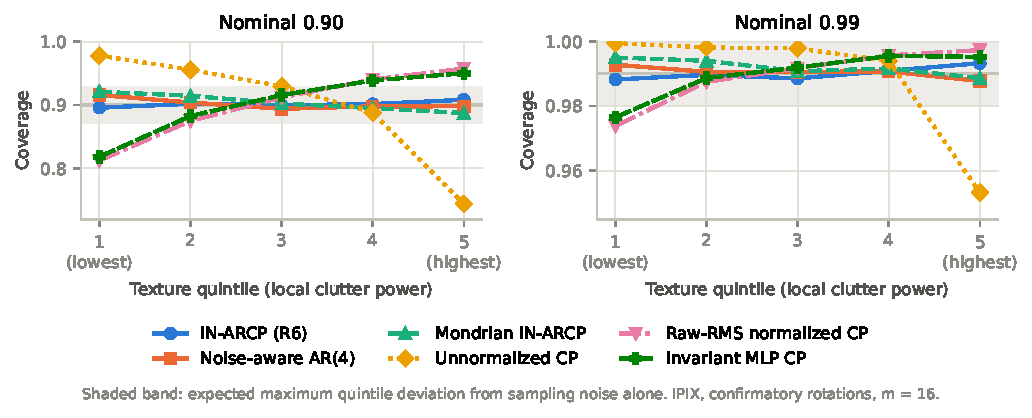
\includegraphics[width=.95\textwidth]{fig_texture_conditional.pdf}
\caption{Coverage by texture quintile on IPIX (confirmatory rotations, $m=16$). Texture is proxied by the local clutter power ($\pm1024$ pulses, excluding the episode).}
\label{fig:texture}
\end{figure*}

\begin{figure*}[t]
\centering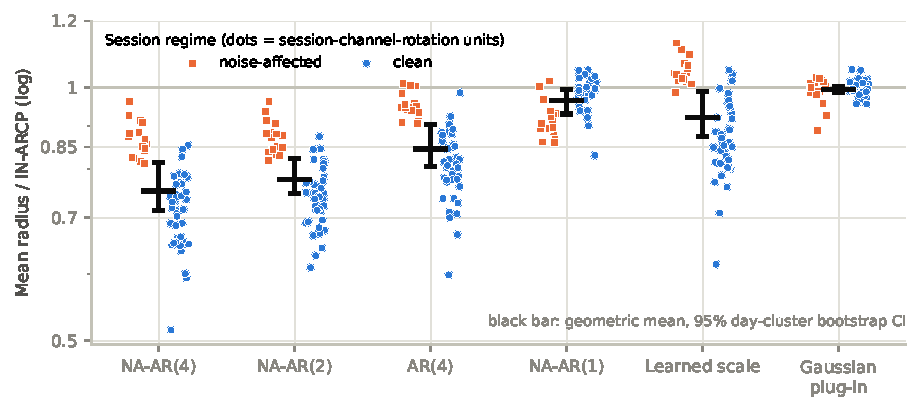
\includegraphics[width=.95\textwidth]{fig_width_ratios.pdf}
\caption{Per-unit radius relative to IN-ARCP at $1-\alpha=0.90$, $m=16$, by session regime (noise-affected: fitted noise power above 1\% of mean power).}
\label{fig:width}
\end{figure*}

\begin{figure*}[t]
\centering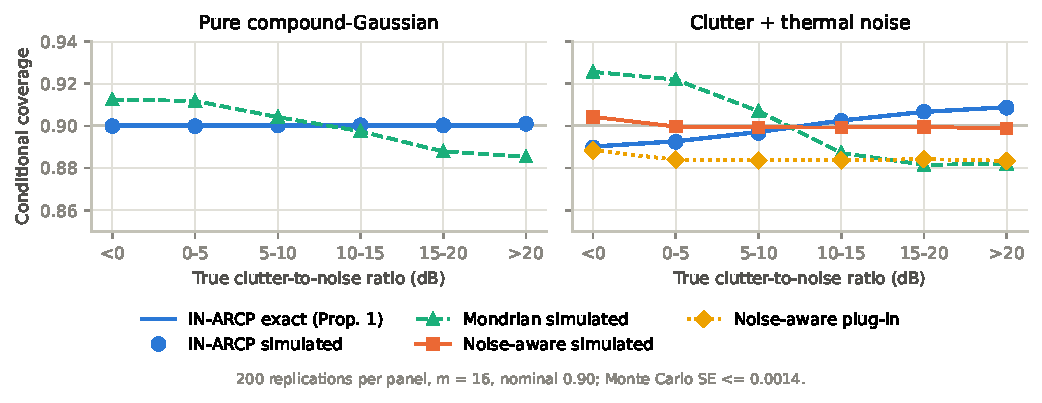
\includegraphics[width=.95\textwidth]{fig_synthetic_exact.pdf}
\caption{Synthetic verification: coverage conditional on the true clutter-to-noise ratio. The line is the exact law of Proposition~\ref{prop:law}; markers are simulation.}
\label{fig:synthetic}
\end{figure*}

\begin{figure*}[t]
\centering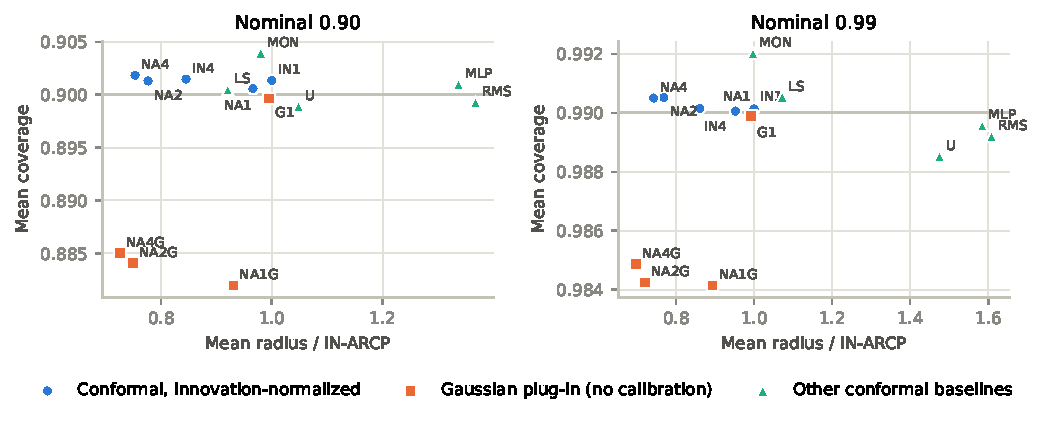
\includegraphics[width=.95\textwidth]{fig_coverage_size.pdf}
\caption{Mean coverage against mean radius (confirmatory, $m=16$). Gaussian plug-ins of the richer noise-aware models are shorter but under-cover; conformal calibration restores nominal coverage.}
\label{fig:covsize}
\end{figure*}

\begin{table}[t]
\centering\footnotesize
\caption{Day transfer ($m=16$, $1-\alpha=0.90$): fit and calibrate on other days, test on each of six held-out days.}
\label{tab:transfer}
\resizebox{\columnwidth}{!}{\begin{tabular}{lccc}
\toprule
Method & Mean coverage & Worst held-out day & Radius ratio\\
\midrule
Noise-aware AR(4) (proposed) & 0.898 & 0.863 & 0.936\\
Noise-aware AR(2) (proposed) & 0.898 & 0.883 & 0.956\\
AR(4), innovation-normalized & 0.901 & 0.894 & 0.993\\
AR(2), innovation-normalized & 0.899 & 0.891 & 1.024\\
Noise-aware AR(1) & 0.900 & 0.882 & 1.037\\
IN-ARCP, AR(1) [R6] & 0.903 & 0.882 & 1.000\\
Gaussian plug-in of IN-ARCP & 0.906 & 0.893 & 1.006\\
Mondrian IN-ARCP & 0.907 & 0.881 & 0.984\\
Learned-scale CP & 0.898 & 0.774 & 0.967\\
Invariant MLP CP & 0.880 & 0.622 & 1.200\\
Raw-RMS normalized CP & 0.906 & 0.681 & 1.466\\
Unnormalized CP & 0.909 & 0.716 & 1.470\\
Gaussian plug-in of NA4 & 0.876 & 0.842 & 0.893\\
\bottomrule
\end{tabular}
}
\end{table}

\begin{table}[t]
\centering\footnotesize
\caption{Hold-out sessions \#269 and \#287 ($1-\alpha=0.90$; six units per column, about 165 test episodes each). Directional check.}
\label{tab:holdout}
\resizebox{\columnwidth}{!}{\begin{tabular}{lcccc}
\toprule
 & \multicolumn{2}{c}{$m=8$} & \multicolumn{2}{c}{$m=16$}\\
\cmidrule(lr){2-3}\cmidrule(lr){4-5}
Method & Radius ratio & Coverage (min) & Radius ratio & Coverage (min)\\
\midrule
Noise-aware AR(4) (proposed) & 0.454 & 0.890 (0.816) & 0.498 & 0.893 (0.847)\\
Noise-aware AR(2) (proposed) & 0.541 & 0.887 (0.828) & 0.533 & 0.895 (0.859)\\
AR(4), innovation-normalized & 0.546 & 0.908 (0.847) & 0.515 & 0.906 (0.883)\\
AR(2), innovation-normalized & 0.582 & 0.905 (0.840) & 0.572 & 0.906 (0.871)\\
Noise-aware AR(1) & 0.921 & 0.898 (0.840) & 0.921 & 0.903 (0.859)\\
IN-ARCP, AR(1) [R6] & 1.000 & 0.906 (0.853) & 1.000 & 0.910 (0.859)\\
Gaussian plug-in of IN-ARCP & 1.178 & 0.949 (0.896) & 1.104 & 0.945 (0.895)\\
Mondrian IN-ARCP & 1.000 & 0.895 (0.804) & 0.981 & 0.896 (0.810)\\
Learned-scale CP & 0.629 & 0.893 (0.804) & 0.662 & 0.919 (0.791)\\
Invariant MLP CP & 1.809 & 0.884 (0.736) & 2.158 & 0.903 (0.761)\\
Raw-RMS normalized CP & 1.321 & 0.880 (0.706) & 1.243 & 0.887 (0.706)\\
Unnormalized CP & 1.142 & 0.868 (0.607) & 1.161 & 0.859 (0.589)\\
Gaussian plug-in of NA4 & 0.411 & 0.866 (0.816) & 0.472 & 0.856 (0.755)\\
\bottomrule
\end{tabular}
}
\end{table}

\section{Conclusion}
For compound-Gaussian radar clutter, innovation normalization makes split-conformal prediction discs texture-conditionally valid in the pure-clutter model. On real sea clutter it keeps them close to that target, where amplitude-equivariant but non-innovation scores do not. Exact complex quadratic-form laws quantify the departure caused by thermal noise and predict cross-day coverage. A noise-aware extension shortens the regions by about a quarter within a session while conformal calibration keeps coverage, which its Gaussian plug-in does not. Extensions to other radars and campaigns, finite-sample versions of the conditioning result, and detection statistics built on these regions remain open.

\section*{Code and data availability}
Code, the frozen protocol, per-episode outcome hashes and figure scripts are in the project repository. The IPIX data are publicly available from McMaster University \cite{ipixweb}.

\section*{Acknowledgment}
% AUTHORS: confirm or edit this disclosure before submission. It must accurately describe who did what.
The authors acknowledge the McMaster University IPIX radar group for making the Dartmouth database available. Generative AI tools assisted this work. OpenAI Codex assisted the earlier revisions (manuscript editing, literature organization, and implementation and verification code). Anthropic Claude assisted this revision with literature checks, derivations, implementation, the design and execution of the pre-registered real-data and synthetic studies, and drafting. [AUTHORS: state here which derivations, analyses and text the authors independently verified.] The authors take full responsibility for the content.

\bibliographystyle{IEEEtran}
\bibliography{references_r7}
\phantomsection
% Restored from the original manuscript, without introducing new author claims.
\begin{IEEEbiography}[{\includegraphics[width=1in,height=1.25in,clip,keepaspectratio]{figures/umair_original_portrait.png}}]{Muhammad Umair Raza}
received the B.E. degree in avionics engineering from NUST, Pakistan, in 2008. He completed his M.S. studies in avionics engineering (signal and image processing) at Air University, Islamabad, in 2015; the degree was conferred in 2017. He is with the Department of Avionics Engineering, College of Aeronautical Engineering, NUST, Risalpur, Pakistan. His work includes signal processing and sensing systems.
\end{IEEEbiography}
\begin{IEEEbiographynophoto}{Sohail Ahmed}
received a degree in avionics engineering from the College of Aeronautical Engineering, Pakistan, the M.S. degree in telecommunications engineering from NUST, Pakistan, and the Ph.D. degree from the University of Southampton, UK. He is a Senior Application Engineer with MathWorks, USA. His research includes communications and radar signal processing.
\end{IEEEbiographynophoto}
\begin{IEEEbiographynophoto}{Ammad Ahmed}
studied aeronautical engineering (avionics) at the National University of Sciences and Technology, Pakistan. He is an RF Engineer with NDMA, Pakistan.
\end{IEEEbiographynophoto}

\EOD
\vfill
\end{document}
